\section{ SR03GB22 }


\subsection{Meta}

    \textbf{Title:}
    The effect of overlapping surgical scheduling on operating theatre productivity: a narrative review

    \begin{table}[H]
        \centering
        \begin{tabular}{|c|c|c|c|c|c|c|c|c|}
            \hline
                \textbf{Rank} & \textbf{Grasp} & \textbf{Grade} & \textbf{Type} & \textbf{Outcome} & \textbf{Domain} & \textbf{COV19} & \textbf{CoI} & \textbf{DB} \\
            \hline
                3 & 98\% & A & A & N & S & Yes & Yes & No \\
            \hline
        \end{tabular}
        \caption{Reference's metadata}
        \label{tab:SR03GB22}
    \end{table}

\subsection{Summary}
    J. J. Pandit, S. K. Ramachandra, and M. Pandit \cite{x333} analysed the theory about productivity increase in surgery operations when using overlapping scheduling of the surgeries. Theoretical and practical research show that the overlapping policy is less effective requires more training and coordination among medical personnel, and, in some cases, increases the risks of surgery complications. In addition, the authors described some differences between US and UK surgery practices and the importance of the turnover time for operational theatre scheduling efficiency. This narrative review is well structured. It contains clear examples and explanations.
    

\subsection{Notes}
    \begin{itemize}
        \item UK NHS;
        \item Massachusetts General Hospital paid > €31 million for use of overlapping scheduling policy;
        \item COVID19 concequence > 6 million patients in waiting list;
        \item UK `Getting it Right First Time` (GIRFT) initiative;
        \item Turnover time = 15\% = 72min in 8-h list;
        \item Touch/Surgeon contact/Knife-to-skin time;
    \end{itemize}


\subsection{Reading}
    \textbf{Abstract:}
    In this paper, the authors research the assumption of the more efficient time consumtion when overlapping thechnieque of surgery conduct is applied. It was discovered that it may be some benefit when there is a lot of short operations with long time of preparing the operating theatres between surgeries. Nevertheless, such improvement should be considered only when the safety, ethical and training conserns are preserved. 
    
    \textbf{Objectives:}
    Analyse the effect of overlapping surgeries in scope of operation theatre time usage, ethics, training and safety asects.

    \textbf{Page 1-2 (Introduction):}
    Massachusetts General Hospital paid > €31 million for use of overlapping scheduling policy. Overlapping is a parallerl surgery between two operating theatres where asistans surgeons operate on non-critical part of the surgery and one lead surgeon provides a critical part of the surgeries. This policy was applyied in response to increased waiting lists after COVID-19 pandemics to over 6 million patients. There is difficulty of defining what is a critical part of the surgery. In addition to overlapping technique the "concurrent" or "simultaneous" policy for overgoing surgeries was introduced.
    
    \textbf{Page 2-5 (Theoretical analysis of overlapping surgery models):}
    The motivation behind overlapping surgeries is to improve productivity. So GIRFT initiative targeted this theory. Turnover time is an insurmountable obsticle to 100\% operating theatre time utilisation. The next paragraph describes in details examples of fault assumption about the improvement of theatre utilisation with one surgeon and two operating theatres and even results in much weaker results.
    \underline{Turnover time} = cleaning, paperwork, equipment preparation, mandatory regulations (e.g. 15-min ventilation). If turnover time == 0 OR surgery does need a lead surgeon OR the whole surgery is critical => overlapping is, by definition, not required or impossible. There is also a gap at the start and at the end of the day list of operations if overlapping approach is used.
    \begin{figure}[H]
        \centering
        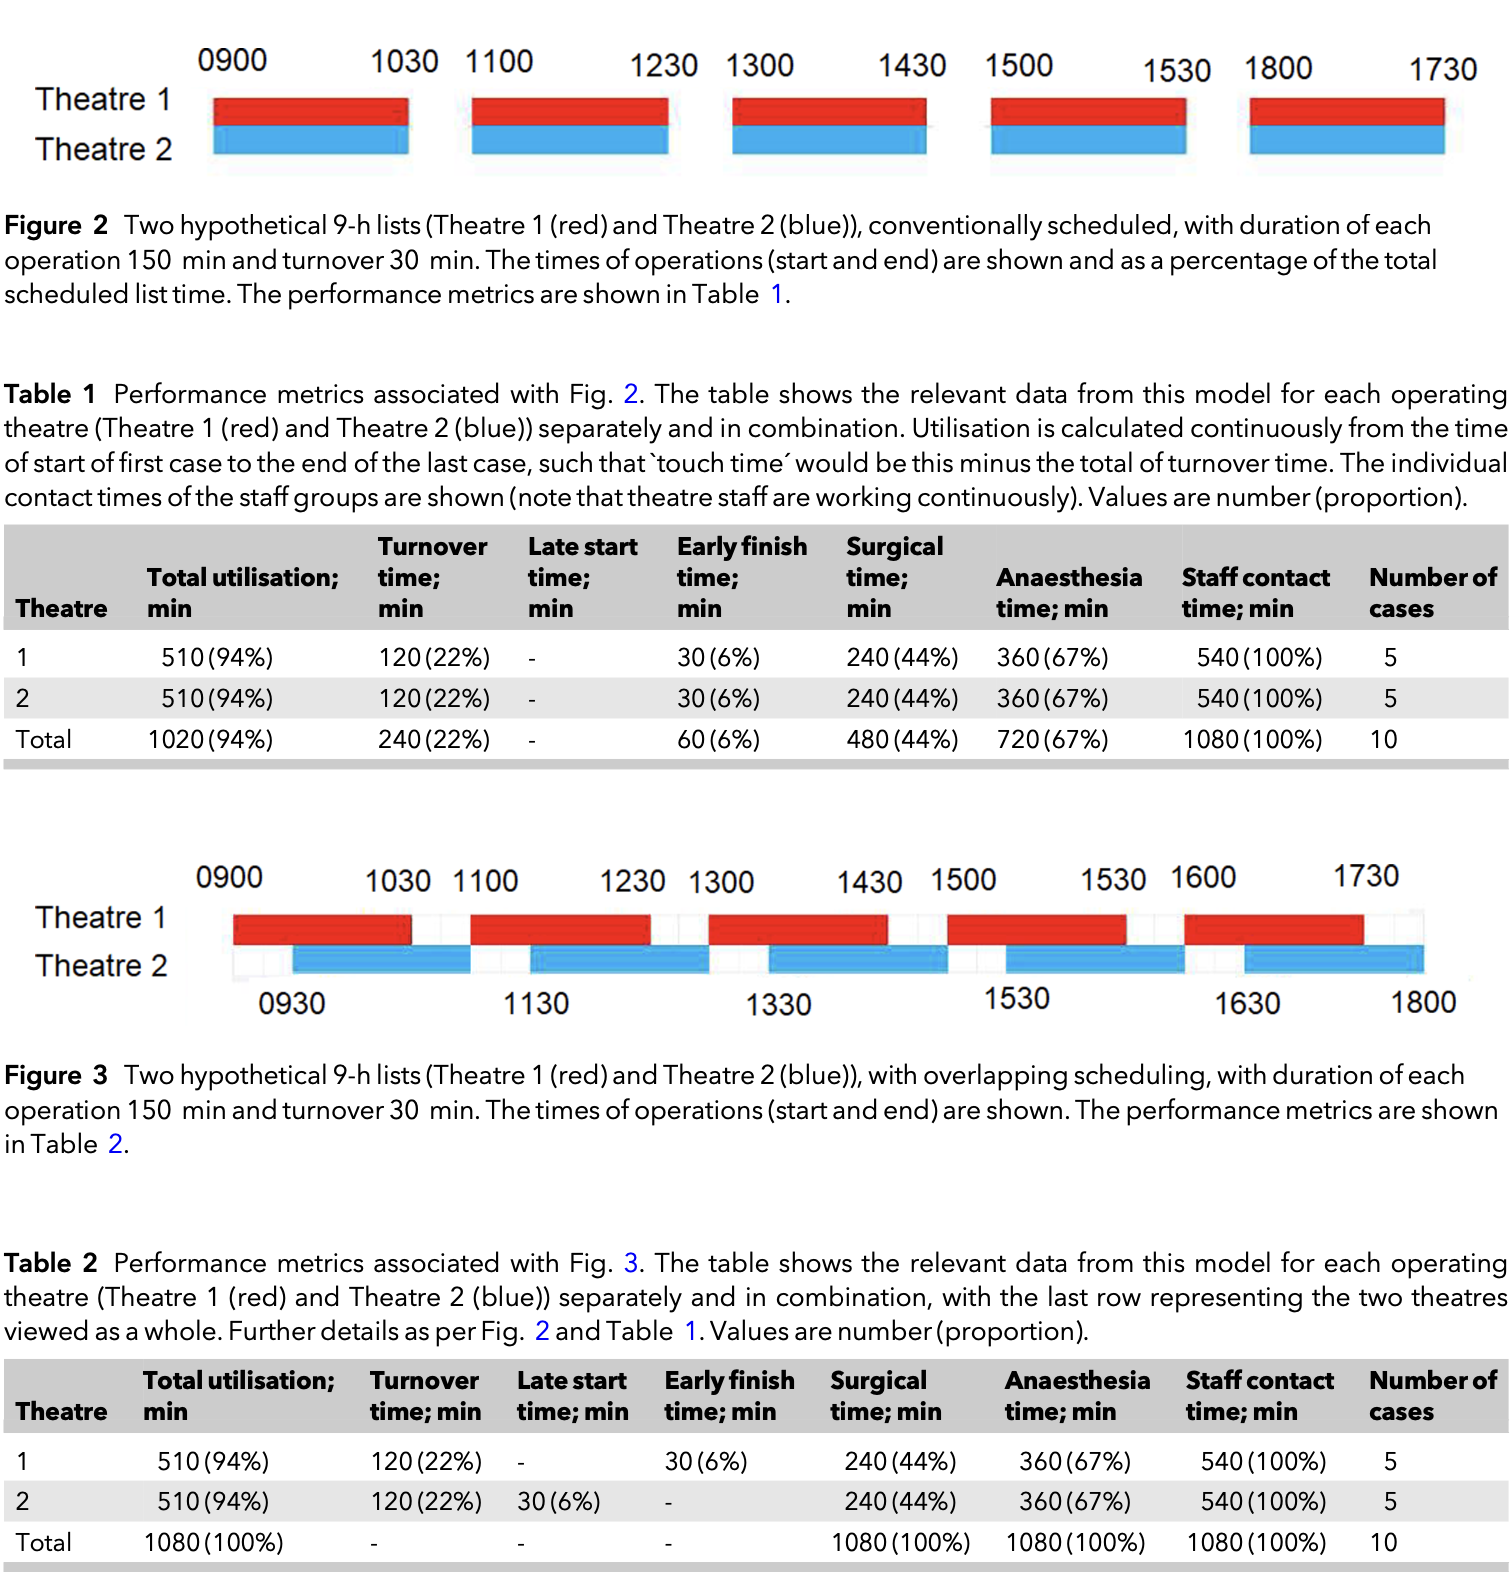
\includegraphics[width=1\textwidth]{figures/0019_SR03GB22/fig1.png}
        \caption{Comparison of parallel and overlapping policies from \cite{x333}.}
        \label{fig1:0019_SR03GB22}
    \end{figure}
    If take US perspective the healthcare industry use billable hours and has disproportionatly high difference between surgeon and other personlle paycheks. But even though, the overlapping does not gain any benefit except making the surgeons busier. Moreover, low level of uncertatinty is crusial for overlapping policy. In conclusion to this section, theoretically the overlapping surgery admission does not provide any benefits over standart parallel surgery practice.

    \textbf{Page 5-6 (Observarional and trial evidence of overlapping surgery):}
    \underline{Safety, training, and ethics}: The data shows that patients who did overgo overlapped operations does not feel different to those who went through classic surgery. Nevertheless this data is mostly for short overlapping time (~<30min). But other findings show that longer overlaps increase chanses to surgery complications. The training and ethical aspects can also be disturbed by using overlapping ~= concurrent ~= simultaneous approaches.

    \textbf{Page 6 (Productivity and costs savings):}
    The single-tunalling on knife-to-skin time improvement damages the overal perseption of the effective healthcare management in overal theatre utilisation time and hospital expances. 

    \textbf{Page 7 (Comparison of different healthcare environments):}
    The overlapping surgery policy increase presure on healthcare management, therefore the geins from implementing it should pay for the efforts. UK - surgery-theatre fix allocation; US - flexible theatre allocation. The overlapping surgery scheduling has not-prooved advantages for temporal application in teams with shortage of staff. The main metric to consider when improving productivity of the operating theatre utilisation is average turnover time. Finally, in order to implement the overlapping approach to conducting surgeries the medical proffesionals should be trained and all risks and ethics should be taken into account. 